\subsection{Stakeholder-Analyse}
Als wesentliche Stakeholder für die Case-Study wurden folgende Parteien ermittelt:

\begin{itemize}
  \item \textbf{Team} - Das Team, welches die Case-Study durchführt ist für die gesamte Planung, Durchführung und Auswertung des Projekts verantwortlich. Es hat sehr grosses Interesse am Gelingen dieses Projektes.
  \item \textbf{Kommiltonen} - Die Kommiltonen arbeiten gleichzeitig an Projekten mit den selben Anforderungen. Sie können das Projekt zwar nicht direkt, jedoch indirekt durch den Austausch von Ideen und Problemen beeinflussen
  \item \textbf{Dozent} - Der Dozent hat durch das Stellen - und allenfalls Verändern - der Aufgabenstellung einen massgeblichen Einfluss auf den Erfolg des Projekts. Dies wird bei dieser Case-Study allerdings dadurch limitiert, dass eine Änderung der Anforderungen nach Projektbeginn ausgeschlossen ist.
  \item \textbf{IBZ} - Die IBZ Schulen AG haben ein relativ geringes Interesse am Projekt an sich, haben aber insofern einen grossen Einfluss darauf, als dass das Projekt abgebrochen werden würde, sollte dies von der Schule verlangt werden. Dieses Szenario ist extrem unrealistisch.
\end{itemize}

\vspace{5mm}

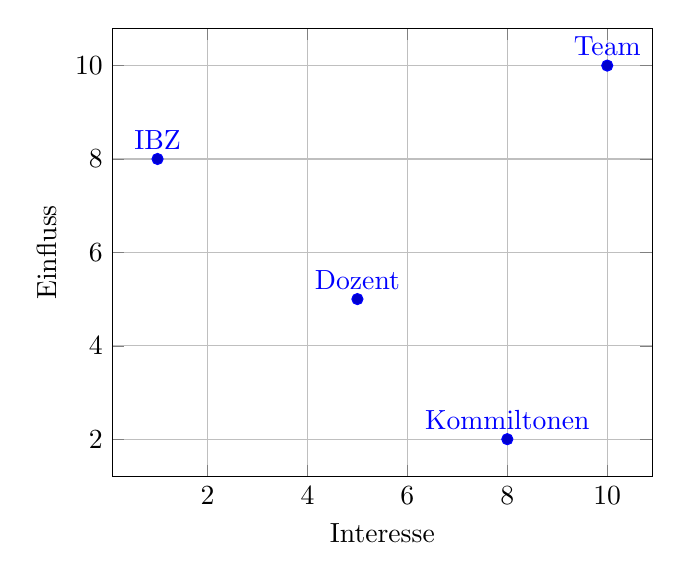
\begin{tikzpicture}
  \begin{axis}[xlabel=Interesse, ylabel=Einfluss, grid=major]
    \addplot+ [nodes near coords,only marks,
    point meta=explicit symbolic]
    table [meta=label] {
    x y label
    10 10 Team
    8 2 Kommiltonen
    5 5 Dozent
    1 8 IBZ
    };
	\end{axis}
\end{tikzpicture}
